% =====================================================================
%  CSE499A — AI Medical Pre-Screening Assistant
%  Standalone section: Project Design (Updated)
%  Reflects enhanced roadmap: 15-module conversational pre-screening pipeline
%  Authors: Rafiur Rahman Mashrafi (2221971042),
%           M.G. Rabbi Hossen (2222516042),
%           Israt Zaman Srity (2211084042)
%  Advisor: Dr. Mohammad Ashrafuzzaman Khan [AzK]
%  Department of Electrical and Computer Engineering,
%  North South University · Spring 2026
% =====================================================================

\documentclass[12pt,a4paper]{article}

\usepackage[utf8]{inputenc}
\usepackage[T1]{fontenc}
\usepackage{mathptmx}
\usepackage[a4paper,margin=1in]{geometry}
\usepackage{setspace}
\usepackage{enumitem}
\usepackage{booktabs}
\usepackage{longtable}
\usepackage{tabularx}
\usepackage{ragged2e}
\usepackage{array}
\usepackage{tikz}
\usepackage[hidelinks]{hyperref}
\usepackage{titlesec}
\usepackage{xcolor}
\usepackage{caption}
\usepackage{mdframed}
\usepackage{amssymb}

\usetikzlibrary{shapes,shapes.geometric,arrows,arrows.meta,positioning,fit,backgrounds}

\onehalfspacing
\setlength{\parskip}{6pt}
\setlength{\parindent}{1.5em}

\titleformat{\section}{\normalfont\large\bfseries}{\thesection}{0.7em}{}
\titleformat{\subsection}{\normalfont\normalsize\bfseries}{\thesubsection}{0.7em}{}

% Framed box for design comparison
\newmdenv[
  backgroundcolor=blue!4,
  linecolor=blue!40,
  linewidth=0.8pt,
  innerleftmargin=8pt,
  innerrightmargin=8pt,
  innertopmargin=6pt,
  innerbottommargin=6pt,
  skipabove=8pt,
  skipbelow=4pt
]{designbox}

\title{\bfseries Project Design (Updated for CSE499B Final Submission):\\
AI Medical Pre-Screening Assistant\\
\large\normalfont\textit{From a 5-Stage ASR Pipeline to a 15-Module
Conversational Clinical Intelligence System}}
\author{Rafiur Rahman Mashrafi (ID 2221971042)\\
        M.~G.~Rabbi Hossen (ID 2222516042)\\
        Israt Zaman Srity (ID 2211084042)\\[6pt]
        \emph{Faculty Advisor:} Dr. Mohammad Ashrafuzzaman Khan [AzK]\\
        Department of Electrical and Computer Engineering\\
        North South University, Bangladesh}
\date{Senior Design Project (CSE499A) \quad Spring 2026}

\begin{document}
\maketitle
\tableofcontents
\newpage

% =====================================================================
\section{Introduction}
% =====================================================================

This chapter presents the updated project design of the
\textit{AI Medical Pre-Screening Assistant}, a system designed to enable
patients --- particularly in Bangladesh --- to describe their symptoms
verbally in Bangla, Banglish, or regional dialects, and to receive a
structured clinical pre-screening report that the attending physician
can review before the consultation begins.

The design presented here is a significant evolution from the
five-stage pipeline described in the original CSE499A proposal. Based
on empirical benchmarks completed during Phases~1--3 of the project,
feedback from the faculty advisor, and a critical review of clinical
requirements, the system has been redesigned from a passive transcription
pipeline into an active, conversational, multi-module clinical
intelligence system. The remainder of this chapter explains what changed,
why it changed, and how the new architecture is organised.

The design is presented in three layers: (i)~the updated 15-module
system architecture that turns a patient's spoken complaint into a
structured, physician-ready pre-screening report; (ii)~the hardware and
software components used to realise the pipeline; and (iii)~the
implementation methodology across the five operational phases of
CSE499A.

\textbf{Important disclaimer:} This system is a pre-screening and
decision-support tool, not a diagnostic system. All outputs are intended
to assist qualified physicians, not replace clinical judgement. Emergency
detection flags are alerts, not diagnoses. Risk levels are probabilistic
classifications, not medical determinations. Final medical decisions
remain entirely with the attending physician.

% =====================================================================
\section{Evolution from the Previous Design}
\label{sec:evolution}
% =====================================================================

\subsection{What the original design was}

The original CSE499A design described a five-stage linear pipeline:

\begin{enumerate}[leftmargin=*]
  \item \textbf{Patient Speech Capture} --- voice recorded on a tablet or kiosk.
  \item \textbf{Automatic Speech Recognition (ASR)} --- Bangla-tuned
        transcription of the recording.
  \item \textbf{Medical Named Entity Recognition (NER)} --- extraction of
        symptoms, medications, durations, allergies, and anatomical sites
        from the transcript.
  \item \textbf{Structured EHR Construction} --- packaging of labelled
        spans into a structured record.
  \item \textbf{Doctor Dashboard with Differential Hints} --- physician
        review interface displaying the record and lightweight diagnostic
        hints.
\end{enumerate}

This was a single-pass, stateless pipeline: the patient spoke once, the
system transcribed and extracted once, and a report was generated from
that single input. There was no mechanism for detecting missing
information, no risk stratification, no follow-up dialogue, and no
emergency triage pathway.

\subsection{What the empirical results revealed}

The Phase~1--3 benchmarks demonstrated that even the strongest
open-source Bangla ASR model (BengaliAI Regional) achieves only
46.94\% WER on real dialect speech, meaning that approximately half of
all words are mis-transcribed. Larger multimodal audio language models
(1.7B--7B parameters) performed significantly worse. This finding has a
direct consequence for system design: if the upstream transcript is
noisy, a single-pass extraction pipeline will silently miss clinical
information with no mechanism to recover it. A patient who mentions a
critical symptom in a poorly-recognised segment will have that symptom
absent from the report.

This realisation, combined with clinical requirements gathered during
Phase~5 (comparative chatbot study), led to the conclusion that the
system must be \textit{interactive}, not passive. Rather than extracting
once from a noisy transcript, the system should identify what is
missing and ask targeted follow-up questions to fill those gaps.

\subsection{Key differences between old and new design}

Table~\ref{tab:comparison} summarises the principal structural
differences between the original five-stage design and the updated
fifteen-module design.

\renewcommand{\arraystretch}{1.3}
\footnotesize
\begin{longtable}{>{\raggedright\arraybackslash}p{3.8cm}
                  >{\raggedright\arraybackslash}p{4.9cm}
                  >{\raggedright\arraybackslash}p{4.9cm}}
\caption{Comparison of original and updated system designs.}
\label{tab:comparison}\\
\toprule
\textbf{Dimension} & \textbf{Original 5-Stage Design} & \textbf{Updated 15-Module Design} \\
\midrule
\endfirsthead
\multicolumn{3}{c}{\itshape Table~\ref{tab:comparison} continued}\\
\toprule
\textbf{Dimension} & \textbf{Original 5-Stage Design} & \textbf{Updated 15-Module Design} \\
\midrule
\endhead
\midrule\multicolumn{3}{r}{\itshape continued\ldots}\endfoot
\bottomrule\endlastfoot
Interaction model
  & Single-pass, stateless. Patient speaks once; system processes once.
  & Conversational, stateful. System identifies gaps and conducts targeted follow-up dialogue. \\
Missing information handling
  & Not addressed. Silent omissions passed to the doctor.
  & Explicit gap detection (Module 6) followed by dynamic follow-up generation (Module 7) in a feedback loop (Modules 8--9). \\
Emergency detection
  & Not present.
  & Dedicated parallel module (Module 5) with rule-based and AI classifier; immediate escalation pathway. \\
Risk stratification
  & Not present (only differential hints).
  & Four-tier risk assessment (Low / Medium / High / Critical) with weighted clinical rules (Module 10). \\
Explainability
  & Not present.
  & Dedicated XAI module (Module 11) generating plain-language explanations of risk assignment (SHAP/LIME or rule traces). \\
Clinical report
  & Structured EHR record with differential hints.
  & Full pre-screening report: chief complaint, symptoms, emergency flags, F/U Q\&A, risk level, possible condition categories, recommended next steps. \\
Language coverage
  & Bangla and Bangla--English code-mixed.
  & Bangla, Banglish, regional dialects. Follow-up questions generated in Bangla or English as appropriate. \\
Feedback loop
  & Not present.
  & Module 15 collects structured doctor feedback for continuous model retraining. \\
Auditability
  & Audio traceable to transcript; transcript visible on dashboard.
  & Full session stored in EHR (Module 13): transcripts, extracted data, follow-up exchanges, risk assessments, reports; versioned overrides. \\
\end{longtable}
\normalsize

% =====================================================================
\section{Updated System Architecture: 15-Module Pipeline}
\label{sec:architecture}
% =====================================================================

\subsection{Architectural overview}

The updated system is organised as a fifteen-module pipeline. The
pipeline is no longer strictly linear: Module~5 (Emergency Detection)
runs in parallel with the main flow; Modules~7--9 form a conditional
feedback loop; and Module~13 (EHR Database) is a persistent store
written to at multiple points. Figure~\ref{fig:fullpipeline} shows the
complete flow.

\begin{figure}[h!]
\centering
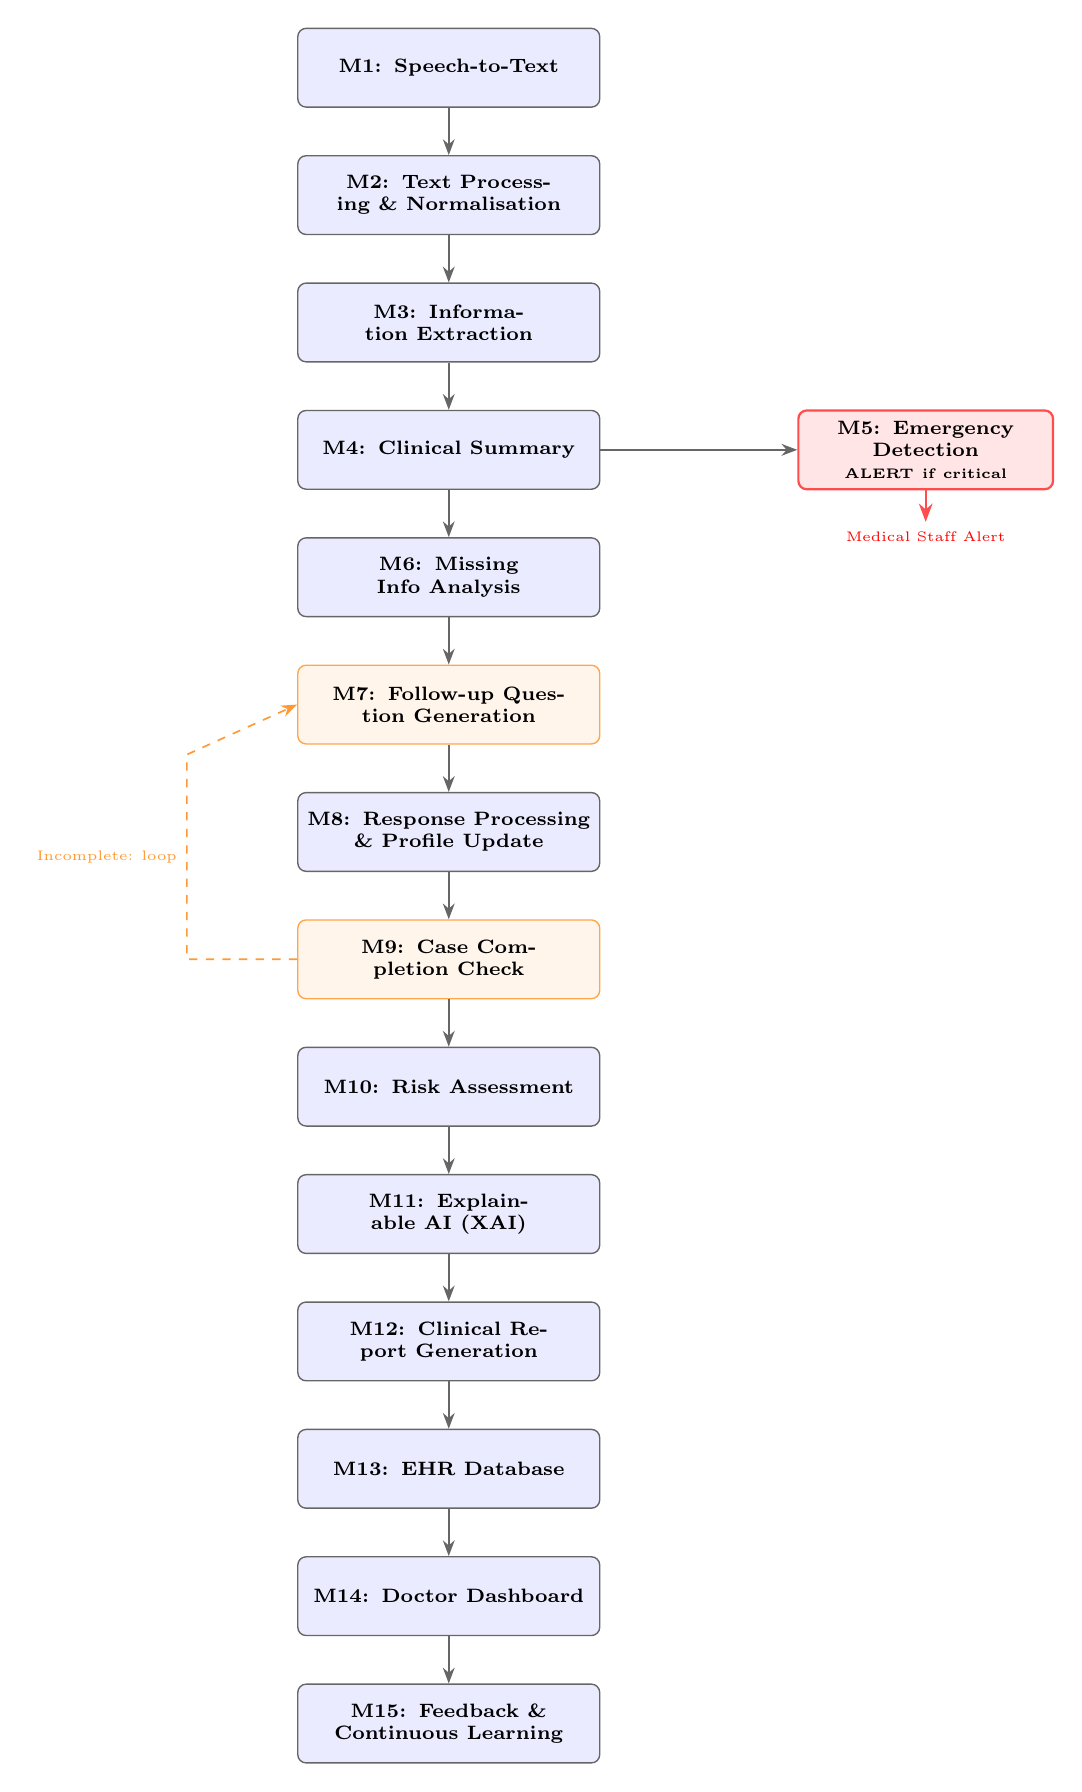
\begin{tikzpicture}[
  node distance=6mm and 5mm,
  mod/.style={rectangle, rounded corners=3pt, draw=black!60,
              fill=blue!8, line width=0.5pt,
              text width=36mm, minimum height=10mm,
              align=center, font=\scriptsize\bfseries},
  alert/.style={rectangle, rounded corners=3pt, draw=red!70,
               fill=red!10, line width=0.8pt,
               text width=30mm, minimum height=10mm,
               align=center, font=\scriptsize\bfseries},
  loop/.style={rectangle, rounded corners=3pt, draw=orange!70,
               fill=orange!8, line width=0.5pt,
               text width=36mm, minimum height=10mm,
               align=center, font=\scriptsize\bfseries},
  arrow/.style={-Stealth, line width=0.6pt, black!60},
  redarrow/.style={-Stealth, line width=0.8pt, red!70},
  loopback/.style={-Stealth, line width=0.6pt, orange!80, dashed}
]
% Main column
\node[mod]                      (m1)  {M1: Speech-to-Text};
\node[mod, below=of m1]         (m2)  {M2: Text Processing \& Normalisation};
\node[mod, below=of m2]         (m3)  {M3: Information Extraction};
\node[mod, below=of m3]         (m4)  {M4: Clinical Summary};
\node[mod, below=of m4]         (m6)  {M6: Missing Info Analysis};
\node[loop, below=of m6]        (m7)  {M7: Follow-up Question Generation};
\node[mod, below=of m7]         (m8)  {M8: Response Processing \& Profile Update};
\node[loop, below=of m8]        (m9)  {M9: Case Completion Check};
\node[mod, below=of m9]         (m10) {M10: Risk Assessment};
\node[mod, below=of m10]        (m11) {M11: Explainable AI (XAI)};
\node[mod, below=of m11]        (m12) {M12: Clinical Report Generation};
\node[mod, below=of m12]        (m13) {M13: EHR Database};
\node[mod, below=of m13]        (m14) {M14: Doctor Dashboard};
\node[mod, below=of m14]        (m15) {M15: Feedback \& Continuous Learning};

% Emergency module to the right
\node[alert, right=25mm of m4]  (m5)  {M5: Emergency\\Detection\\{\tiny ALERT if critical}};

% Main arrows
\draw[arrow] (m1)--(m2);
\draw[arrow] (m2)--(m3);
\draw[arrow] (m3)--(m4);
\draw[arrow] (m4)--(m6);
\draw[arrow] (m6)--(m7);
\draw[arrow] (m7)--(m8);
\draw[arrow] (m8)--(m9);
\draw[arrow] (m9)--(m10);
\draw[arrow] (m10)--(m11);
\draw[arrow] (m11)--(m12);
\draw[arrow] (m12)--(m13);
\draw[arrow] (m13)--(m14);
\draw[arrow] (m14)--(m15);

% Emergency branch
\draw[arrow]    (m4.east) -- (m5.west);
\draw[redarrow] (m5.south) -- ++(0,-4mm) node[below,font=\tiny,red]{Medical Staff Alert};

% Loop-back arrow from M9 to M7
\draw[loopback] (m9.west) -- ++(-14mm,0) -- ++(0,26mm) node[midway,left,font=\tiny,orange!80]{Incomplete: loop} -- (m7.west);

\end{tikzpicture}
\caption{Complete 15-module pipeline of the AI Medical Pre-Screening Assistant. Orange loop indicates the
follow-up question cycle; red branch is the emergency escalation pathway.}
\label{fig:fullpipeline}
\end{figure}

\subsection{Module 1: Speech-to-Text}
\label{sec:m1}

\textbf{Goal:} Convert patient voice input into raw text.

The patient speaks freely in Bangla, Banglish, or a regional dialect.
A speech recognition model trained or fine-tuned on Bangladeshi speech
patterns handles transcription. The module must tolerate ambient noise,
strong accents, and code-switching between Bangla and English. If
speech quality falls below a configurable threshold, the system falls
back to a manual text-entry interface.

\textbf{Key requirements:} Dialect-aware acoustic model; real-time or
near-real-time transcription; noise-tolerant voice activity detection;
fallback to manual text input.

\textbf{Connection to Phase~1--4 benchmarks:} The empirical work
completed during CSE499A directly feeds this module. BengaliAI Regional
(46.94\% WER) is the current strongest baseline; fine-tuning
Qwen3-ASR-1.7B with LoRA on the multi-dialect corpus (scheduled for
CSE499B) is the pathway to a production-grade transcription engine.

\subsection{Module 2: Text Processing and Normalisation}
\label{sec:m2}

\textbf{Goal:} Clean, standardise, and prepare raw transcribed text for
downstream analysis.

This module handles spelling correction, normalisation of Banglish text,
removal of filler words, punctuation restoration, and sentence boundary
detection. Where necessary it translates Bangla or Banglish content into
a standardised form that the rest of the pipeline can process
consistently.

\textbf{Key requirements:} NLP preprocessing pipeline; Bangla--English
bilingual handling; medical spelling correction; noise and artefact
removal.

\subsection{Module 3: Information Extraction}
\label{sec:m3}

\textbf{Goal:} Extract structured clinical data from the normalised
text.

The system identifies and tags key clinical entities including symptoms,
affected body parts, duration, severity, frequency, patient age, and
any pre-existing conditions or medications mentioned. This forms the
foundation of the patient profile.

\textbf{Key requirements:} Medical NLP; named entity recognition for
clinical entities; temporal expression extraction (e.g., ``for three
days'', ``since last week'').

\textbf{Connection to original design:} This module directly extends the
Medical NER stage from the original five-stage pipeline, expanding the
entity set and adding temporal reasoning.

\subsection{Module 4: Initial Clinical Summary Generation}
\label{sec:m4}

\textbf{Goal:} Generate a concise, human-readable summary of the
patient's chief complaint from the extracted entities.

\textbf{Example output:} \textit{``Patient reports fever and dry cough
for 3 days, with mild fatigue. No mention of breathing difficulty or
chest pain.''}

\textbf{Key requirements:} Medical text summarisation model; templated
and generative output options.

\subsection{Module 5: Emergency Detection}
\label{sec:m5}

\textbf{Goal:} Immediately flag life-threatening or urgent conditions
before the full pipeline runs.

This module runs in parallel with or immediately after extraction. It
checks for red-flag symptoms --- chest pain, stroke indicators, severe
breathing difficulty, loss of consciousness, acute trauma --- and
triggers an immediate alert if any are detected. This module has
absolute priority over all others.

\textbf{Key requirements:} Rule-based critical symptom checker; AI
classifier for ambiguous emergency presentations; escalation pathway to
alert medical staff immediately.

\textbf{New in updated design:} Emergency triage was completely absent
from the original architecture. Its addition was driven by clinical
safety requirements identified during the Phase~5 chatbot study.

\subsection{Module 6: Missing Information Analysis}
\label{sec:m6}

\textbf{Goal:} Identify clinical information gaps that are necessary for
a complete pre-screening profile.

Using clinical reasoning rules and medical knowledge, the system checks
what information is present versus what is expected and produces a
structured gap report.

\textbf{Example output:}
\begin{itemize}[leftmargin=*, noitemsep]
  \item[\checkmark] Symptom detected: Fever
  \item[$\times$] Temperature reading not provided
  \item[$\times$] Duration of fever not specified
  \item[$\times$] Breathing difficulty not assessed
\end{itemize}

\textbf{Key requirements:} Symptom completeness logic; clinical
checklists per condition category; structured gap report generation.

\textbf{New in updated design:} This module is the principal motivation
for moving from a single-pass to a conversational architecture. ASR
errors in Module~1 mean that a single pass will routinely miss clinical
information; Module~6 makes those omissions explicit rather than letting
them propagate silently to the physician.

\subsection{Module 7: Dynamic Follow-up Question Generation}
\label{sec:m7}

\textbf{Goal:} Generate targeted, conversational questions to fill the
identified information gaps.

Questions are generated in natural language --- in Bangla or English as
appropriate --- prioritised by clinical importance, and adapted to avoid
redundancy with information already collected.

\textbf{Example output:} \textit{``Apnar jwor ki matro kal theke?
Thermometer diye measure korechen?''} / \textit{``When did your fever
start? Have you measured your temperature?''}

\textbf{Key requirements:} Question generation model with medical
context; Bangla/English bilingual output; priority ranking of questions.

\subsection{Module 8: Response Processing and Profile Update}
\label{sec:m8}

\textbf{Goal:} Analyse patient answers to follow-up questions and update
the patient profile.

New answers go through the same extraction and normalisation pipeline as
the original input (Modules~2--3). Extracted information is merged into
the existing patient profile, resolving contradictions and marking
newly filled gaps.

\textbf{Key requirements:} Incremental NLP pipeline; patient profile
state management; conflict resolution logic.

\subsection{Module 9: Case Completion Check}
\label{sec:m9}

\textbf{Goal:} Determine whether sufficient information has been
collected to proceed to assessment.

The system scores the completeness of the patient profile against a
minimum threshold for reliable pre-screening. If critical gaps remain,
it loops back to Module~7. The loop continues until the profile is
sufficiently complete or a configurable maximum number of turns is
reached (to avoid patient fatigue).

\textbf{Key requirements:} Completeness scoring model; configurable
thresholds per condition type; loop management and turn limits.

\subsection{Module 10: Risk Assessment}
\label{sec:m10}

\textbf{Goal:} Classify the patient into a risk tier based on their
complete profile.

The system assigns one of four risk levels using a combination of
clinical decision rules and a trained risk prediction model. Risk
factors such as age, comorbidities, symptom severity, and duration are
all weighted. Critical-risk cases are re-flagged for immediate attention.

\begin{designbox}
\textbf{Risk tiers:}\\[2pt]
\textbf{Low} --- Likely minor, self-limiting condition.\\
\textbf{Medium} --- Warrants examination but not urgent.\\
\textbf{High} --- Needs prompt medical attention.\\
\textbf{Critical} --- Requires immediate intervention.
\end{designbox}

\textbf{Key requirements:} Risk classification model; clinical rule
engine; age/comorbidity weighting; integration with Module~5 output.

\textbf{New in updated design:} The original design offered only
differential hints; structured, four-tier risk stratification with
weighted clinical factors is entirely new.

\subsection{Module 11: Explainable AI (XAI)}
\label{sec:m11}

\textbf{Goal:} Make the system's reasoning transparent and auditable for
physicians and regulators.

For every risk assessment, the system generates a plain-language
explanation of which symptoms, durations, and risk factors contributed
to the classification.

\textbf{Example output:} \textit{``High risk was assigned due to: fever
lasting more than 5 days, reported difficulty breathing, and patient age
over 65.''}

\textbf{Key requirements:} Feature attribution methods (LIME, SHAP, or
rule-based reasoning traces); human-readable explanation generation;
display on the doctor dashboard alongside the report.

\textbf{New in updated design:} Explainability was absent from the
original architecture. Its addition is motivated by medical
accountability requirements and by the clinical need for physicians to
be able to trust and, where necessary, override automated assessments.

\subsection{Module 12: Structured Clinical Report Generation}
\label{sec:m12}

\textbf{Goal:} Compile all collected information into a formatted
pre-screening report ready for the physician.

The report presents a standardised summary that the physician can review
before or during the consultation. It does not contain a diagnosis.

\textbf{Report sections:}
\begin{enumerate}[leftmargin=*, noitemsep]
  \item Patient Profile (age, gender, known conditions)
  \item Chief Complaint
  \item Symptoms with Duration and Severity
  \item Emergency Flags (if any)
  \item Follow-up Questions and Answers
  \item Risk Level and Explanation
  \item Possible Condition Categories (not a diagnosis)
  \item Recommended Next Steps
\end{enumerate}

\textbf{Key requirements:} Medical report generation; structured and
human-readable output; PDF and digital dashboard export options.

\subsection{Module 13: EHR Database}
\label{sec:m13}

\textbf{Goal:} Securely store all patient data, reports, and interaction
history.

Every session --- transcripts, extracted data, follow-up exchanges, risk
assessments, and final reports --- is stored in a structured medical
database. Records are linked to patient identifiers and consultation
timestamps and support future retrieval, audits, and longitudinal
tracking.

\textbf{Key requirements:} Secure, HIPAA/PDPA-compliant database design;
encryption at rest and in transit; patient identity management; efficient
retrieval by patient ID or date; audit logging.

\subsection{Module 14: Doctor Dashboard}
\label{sec:m14}

\textbf{Goal:} Give physicians a clear, fast interface to review the
pre-screening report before or during consultation.

The dashboard displays the structured clinical report, risk level,
emergency flags, and the XAI explanation. Physicians can review the
conversation history, validate or override extracted information, and
add annotations. A notification system alerts physicians to high or
critical risk cases immediately.

\textbf{Key requirements:} Web-based dashboard; role-based access
control; real-time notifications for high/critical cases; annotation and
override tools; mobile-responsive design.

\textbf{Connection to original design:} The doctor dashboard was present
in the original design. The updated version adds risk-tier display,
XAI explanations, real-time critical alerts, and structured override
tools.

\subsection{Module 15: Feedback and Continuous Learning}
\label{sec:m15}

\textbf{Goal:} Use physician feedback to improve system accuracy and
clinical relevance over time.

After each consultation, physicians can rate the quality of the
pre-screening report, correct inaccurate extractions, flag missed
symptoms, and annotate risk-level disagreements. This feedback is
collected, reviewed, and used to retrain or fine-tune the extraction,
risk assessment, and question-generation models.

\textbf{Key requirements:} Structured feedback collection interface;
feedback dataset management; model retraining pipeline; performance
monitoring and regression testing before deploying updated models.

\textbf{New in updated design:} No feedback loop existed in the original
design. Module~15 closes the quality circle and is the mechanism through
which the system improves beyond the CSE499B deployment.

% =====================================================================
\section{System Flow Summary}
\label{sec:flow}
% =====================================================================

\begin{verbatim}
Patient Speaks (Bangla / Banglish / Dialect)
        |
        v
Module 1  -- Speech-to-Text
        |
        v
Module 2  -- Text Processing & Normalisation
        |
        v
Module 3  -- Information Extraction
        |
        v
Module 4  -- Initial Clinical Summary
        |
   +----+----+
   |         |
   v         v
Module 5  Module 6 -- Missing Information Analysis
(Emergency  |
Detection)  v
[ALERT if   Module 7 -- Follow-up Question Generation
critical]   |
            v
       Patient Answers
            |
            v
Module 8  -- Response Processing & Profile Update
            |
            v
Module 9  -- Case Completion Check
   +--------+--------+
   |                 |
   v                 v
[Incomplete]      [Complete]
Loop to M7        Continue
                     |
                     v
Module 10 -- Risk Assessment
                     |
                     v
Module 11 -- Explainable AI (XAI)
                     |
                     v
Module 12 -- Clinical Report Generation
                     |
                     v
Module 13 -- EHR Database (Store)
                     |
                     v
Module 14 -- Doctor Dashboard (Review)
                     |
                     v
Module 15 -- Feedback & Continuous Learning
\end{verbatim}

% =====================================================================
\section{Hardware and Software Components}
\label{sec:components}
% =====================================================================

This remains a software-only project; no custom hardware has been
fabricated. The patient-facing capture device in deployment would be a
consumer Android tablet (8--10\,inch form factor) or a fixed clinic
kiosk. All model evaluation and development was performed on free-tier
Google Colab GPU instances. Table~\ref{tab:tools} lists the principal
software components.

\renewcommand{\arraystretch}{1.2}
\footnotesize
\begin{longtable}{>{\raggedright\arraybackslash}p{2.8cm}
                  >{\raggedright\arraybackslash}p{3.2cm}
                  >{\raggedright\arraybackslash}p{2.5cm}
                  >{\raggedright\arraybackslash}p{4.5cm}}
\caption{Software tools and components.}\label{tab:tools}\\
\toprule
\textbf{Tool} & \textbf{Function} & \textbf{Similar tools} & \textbf{Why this one} \\
\midrule
\endfirsthead
\multicolumn{4}{c}{\itshape Table~\ref{tab:tools} continued}\\
\toprule
\textbf{Tool} & \textbf{Function} & \textbf{Similar tools} & \textbf{Why this one} \\
\midrule
\endhead
\midrule\multicolumn{4}{r}{\itshape continued\ldots}\endfoot
\bottomrule\endlastfoot
Python 3.10 & Implementation language & R, Julia & Standard for ML/NLP; widest ecosystem. \\
PyTorch 2.x & Deep-learning framework & TensorFlow, JAX & Native support across all evaluated ASR models; preferred by Hugging Face. \\
HF Transformers \cite{pd:transformers} & Model loading, inference, tokenisation & ESPnet, NeMo & Unified API across Whisper, Wav2Vec2, MMS, SeamlessM4T, Qwen-Audio. \\
HF PEFT / LoRA \cite{pd:lora} & Parameter-efficient fine-tuning & Full fine-tune, DeepSpeed & Enables fine-tuning Qwen3-ASR-1.7B on free-tier Colab within memory limits. \\
BanglaBERT \cite{pd:banglabert} & Medical NER token classification & mBERT, XLM-R & Pre-trained on Bangla; lowest adaptation cost for clinical NER. \\
spaCy + custom rules & Temporal expression extraction, rule-based clinical checkers & NLTK, Stanford NLP & Fast, production-ready; custom rule layers for Module 6 completeness logic. \\
Librosa / SoundFile / FFmpeg & Audio I/O, resampling, mono conversion & torchaudio, sox & Stable; runs reliably on Colab. \\
WhisperX \cite{pd:whisperx} & Long-form audio segmentation & pyannote.audio & Required for audio longer than Whisper's 30-second window. \\
\texttt{jiwer}, \texttt{evaluate} & WER, CER, BLEU scoring & sclite & Pure-Python; standard for speech evaluation. \\
FastAPI (Python) & REST/WebSocket backend & Flask, Django & Async-native; low latency for conversational follow-up loop. \\
PostgreSQL (encrypted) & EHR store (Module 13) & MySQL, MongoDB & Row-level encryption; relational schema suits structured clinical records. \\
React / Next.js & Doctor dashboard (Module 14) & Vue.js, Angular & Component ecosystem; server-side rendering for low-bandwidth clinics. \\
Flutter / PWA & Patient kiosk front-end (Module 1) & React Native & Single codebase; large Bangla font support; single-button record UX. \\
SHAP / LIME & XAI feature attribution (Module 11) & Integrated Gradients & Model-agnostic; produces human-readable explanations for clinical risk. \\
Google Colab (T4, A100) & Primary GPU compute & Kaggle, local GPU & Free tier sufficient for all CSE499A inference benchmarks. \\
Git / GitHub & Source control & GitLab & Required for reproducibility and submission. \\
\end{longtable}
\normalsize

\subsection{Planned components for the deployed system (CSE499B)}

The CSE499B implementation will add the following components above the
model pipeline:
\begin{itemize}[leftmargin=*]
  \item \textbf{JWT authentication and role-based access control} ---
        distinct roles for patients (no read access), nurses (intake
        only), physicians (full record), administrators (no clinical
        content).
  \item \textbf{PDPA-compliant consent management} --- recorded verbal
        consent integrated into the patient kiosk flow before any
        recording begins.
  \item \textbf{Model retraining pipeline (Module 15)} ---
        MLflow-tracked experiment management for continuous learning
        cycles using physician feedback datasets.
  \item \textbf{PDF report export} --- formatted clinical pre-screening
        report (Module~12) exportable as a PDF for printing or EHR
        attachment.
\end{itemize}

% =====================================================================
\section{Implementation Methodology}
\label{sec:phases}
% =====================================================================

The CSE499A work was organised around five operational phases, each
closed by a demonstration to the faculty advisor.

\subsection*{Phase 1 --- Audio collection and preprocessing}
\textit{Demo 1: 12 March 2026.}
A multi-dialect Bangla audio corpus was assembled from publicly
available recordings covering five regional varieties: Puran Dhaka
(Dhakaiya), Barishali, Sylheti, Normal Bangla, and Indian Bangla.
Each file was renamed under a fixed convention
\texttt{[dialect]\_[index]\_[gender]\_[age].mp3} and logged in
\texttt{dataset\_log.csv} with source, dialect code, speaker gender,
approximate age, and duration. The corpus was preprocessed: resampled
to 16~kHz mono PCM, RMS-normalised, and segmented into 10--15-second
clips by WhisperX's voice-activity detector. The final corpus is
approximately 4.7 hours, 10 source files, $\sim$1{,}100 evaluation
segments.

\subsection*{Phase 2 --- Baseline ASR benchmark (12 models)}
\textit{Demo 2: 2 April 2026.}
Twelve open-source Bangla and multilingual ASR models were benchmarked
on the corpus: Whisper Small/Medium/Large/Turbo, Wav2Vec2 (XLSR-53,
300M, Common-Voice-Bengali variants), MMS, Vakyansh-Bn, BengaliAI
Whisper, BengaliAI Regional, and SeamlessM4T. Each model transcribed
the entire corpus and was scored using WER, CER, and corpus-level BLEU.
The strongest baseline was BengaliAI Regional at 46.94\% WER, 24.29\%
CER, and 0.273 BLEU. The principal finding was that even the strongest
open Bangla model mis-transcribes nearly half of all words on dialect
speech --- the direct motivator for the conversational gap-filling
architecture added in Modules~6--9.

\subsection*{Phase 3 --- Larger multimodal audio LLM benchmark}
\textit{Demo 3: 9 April 2026.}
Six larger 1.7B--7B-parameter multimodal audio language models were
evaluated on the same corpus: Qwen2-Audio (English-routing and direct
Bangla modes), Qwen3-ASR-1.7B, Voxtral-Mini, Phi-4 Multimodal, and
Qwen2.5-Omni. None matched the smaller specialised baseline; the
closest trailed BengaliAI Regional by more than 50 percentage points
of WER. The conclusion --- ``bigger is not better for Bangla dialect
speech'' --- confirms that Module~1 must use a specialised, fine-tuned
model rather than a general-purpose large model.

\subsection*{Phase 4 --- Qwen3-ASR fine-tuning research (in progress)}
\textit{Demo 4: 16 April 2026.}
The team researched the methodology for parameter-efficient fine-tuning
of Qwen3-ASR-1.7B on the multi-dialect corpus, using LoRA adapters on
the speech encoder with the language-model decoder weights frozen. No
training has been performed yet; this phase is a methodology study. The
fine-tuning is scheduled for CSE499B and will produce the production
ASR engine for Module~1.

\subsection*{Phase 5 --- Comparative chatbot output study (selected)}
\textit{Selected: 23 April 2026; execution scheduled for the next demo.}
Several public AI chatbots --- ChatGPT, DeepSeek, Qwen, Perplexity ---
will be prompted with simulated patient utterances. Their structured
EHR-style outputs will be compared along axes of schema consistency,
completeness, handling of code-mixed terms, and source faithfulness.
This phase directly informed the design of Module~12 (clinical report
schema) and Module~6 (information gap taxonomy), and it surfaced the
requirement for emergency triage (Module~5) and explicit risk
stratification (Module~10) that were absent from the original design.

% =====================================================================
\section{Data Privacy and Clinical Safety Constraints}
% =====================================================================

\textbf{Data privacy and consent} must be handled before any recording
begins. Patients are informed in Bangla of how their voice and health
data will be used and stored, and explicit verbal consent is recorded as
part of the session (Module~1). All data is processed under
HIPAA/PDPA-equivalent constraints: encrypted at rest and in transit,
accessible only through role-based controls, and retained for the
minimum period required.

\textbf{Multilingual and dialect coverage} will be continuously expanded
based on real usage data collected through the feedback loop in
Module~15.

\textbf{Clinical safety boundary:} The system outputs a pre-screening
report, not a diagnosis. All clinical decisions remain with the licensed
physician. The risk levels produced by Module~10 are probabilistic
indicators derived from self-reported symptoms; they are not medical
determinations and are not legally equivalent to a clinical assessment.

% =====================================================================
\section{Conclusion}
% =====================================================================

The updated project design presented above represents a fundamental
redesign of the system from a passive, single-pass transcription
pipeline into an active, conversational, fifteen-module clinical
intelligence system. The driving force behind this evolution was
empirical: the Phase~1--3 benchmarks demonstrated that Bangla dialect
ASR at 46.94\% WER is too noisy for a single-pass extraction to be
clinically reliable, and the Phase~5 chatbot study revealed that
multiple critical clinical functions --- emergency triage, risk
stratification, gap detection, and explainability --- were absent from
the original design.

The updated architecture addresses these gaps directly. Module~5 provides
a dedicated emergency escalation pathway. Modules~6--9 form a
conversational loop that closes information gaps before assessment.
Module~10 replaces informal differential hints with a structured,
four-tier risk model. Module~11 makes the system's reasoning auditable.
Module~15 ensures the system improves continuously from physician
feedback. All of these additions serve a single clinical goal: to
give the physician an accurate, complete, and trustworthy pre-screening
report before the consultation begins, so that consultation time is used
for examination and clinical judgement rather than for basic
information-gathering.

The empirical benchmarks of Phases~2 and~3 confirm that
Module~1 must use a specialised, fine-tuned Bangla model
(Qwen3-ASR-1.7B with LoRA, scheduled for CSE499B) rather than a
general-purpose large model. The remainder of the fifteen modules will
be designed, integrated, and validated in CSE499B.

% =====================================================================
\begin{thebibliography}{99}

\bibitem{pd:whisper}
A.~Radford \emph{et al.},
``Robust Speech Recognition via Large-Scale Weak Supervision,''
in \emph{Proc.\ ICML 2023}, pp.~28492--28518.
\url{https://arxiv.org/abs/2212.04356}.

\bibitem{pd:mms}
V.~Pratap \emph{et al.},
``Scaling Speech Technology to 1{,}000+ Languages,''
\emph{arXiv:2305.13516}, 2023.
\url{https://arxiv.org/abs/2305.13516}.

\bibitem{pd:wav2vec2}
A.~Baevski \emph{et al.},
``wav2vec 2.0: A Framework for Self-Supervised Learning of Speech
Representations,''
\emph{NeurIPS}, vol.~33, 2020, pp.~12449--12460.
\url{https://arxiv.org/abs/2006.11477}.

\bibitem{pd:qwen2audio}
Y.~Chu \emph{et al.},
``Qwen2-Audio Technical Report,''
\emph{arXiv:2407.10759}, 2024.
\url{https://arxiv.org/abs/2407.10759}.

\bibitem{pd:transformers}
T.~Wolf \emph{et al.},
``Transformers: State-of-the-Art Natural Language Processing,''
in \emph{Proc.\ EMNLP 2020: System Demonstrations}, pp.~38--45.
\url{https://github.com/huggingface/transformers}.

\bibitem{pd:lora}
E.~J.~Hu \emph{et al.},
``LoRA: Low-Rank Adaptation of Large Language Models,''
in \emph{ICLR 2022}.
\url{https://arxiv.org/abs/2106.09685}.

\bibitem{pd:whisperx}
M.~Bain \emph{et al.},
``WhisperX: Time-Accurate Speech Transcription of Long-Form Audio,''
in \emph{INTERSPEECH 2023}.
\url{https://arxiv.org/abs/2303.00747}.

\bibitem{pd:banglabert}
A.~Bhattacharjee \emph{et al.},
``BanglaBERT: Language Model Pretraining and Benchmarks for
Low-Resource Language Understanding Evaluation in Bangla,''
\emph{Findings of NAACL 2022}, pp.~1318--1327.
\url{https://github.com/csebuetnlp/banglabert}.

\bibitem{pd:oodspeech}
F.~R.~Rakib \emph{et al.},
``OOD-Speech: A Large Bengali Speech Recognition Dataset for
Out-of-Distribution Benchmarking,''
\emph{INTERSPEECH 2023}.
\url{https://arxiv.org/abs/2305.09688}.

\bibitem{pd:shap}
S.~M.~Lundberg and S.-I.~Lee,
``A Unified Approach to Interpreting Model Predictions,''
\emph{NeurIPS}, vol.~30, 2017.
\url{https://arxiv.org/abs/1705.07874}.

\bibitem{pd:lime}
M.~T.~Ribeiro, S.~Singh, and C.~Guestrin,
```Why Should I Trust You?': Explaining the Predictions of Any
Classifier,''
in \emph{Proc.\ KDD 2016}, pp.~1135--1144.
\url{https://arxiv.org/abs/1602.04938}.

\end{thebibliography}

\end{document}